\documentclass[onecolumn, 12pt]{report}
\usepackage{hyperref,mathtools,amssymb}
\usepackage{cite}
\usepackage{graphicx}
\usepackage{xcolor}
\usepackage{subcaption}
\usepackage[margin=0.75in]{geometry}

\title{ERCAP Proposal: rotating bosons via CL with AMReX}
%\subject{Many-Body Quantum Mechanics}
\author{Casey Berger, Don Willcox}
\date{\today}

\newcommand{\note}[1]{{\color{red} \bf[NOTE: #1]}}
\newcommand{\etal}{{\it et al.}}
\newcommand{\beq}{\begin{equation}}
\newcommand{\eeq}{\end{equation}}
\newcommand{\bea}{\begin{eqnarray}}
\newcommand{\eea}{\end{eqnarray}}

\def\CP{{\mathcal P}}
\def\CC{{\mathcal C}}
\def\CH{{\mathcal H}}
\def\CW{{\mathcal W}}
\def\CO{{\mathcal O}}
\def\CZ{{\mathcal Z}}
\def\CD{{\mathcal D}}
\def\del{{\nabla}}

\newcommand*\dif{\mathop{}\!\mathrm{d}}

\begin{document}
\section{Project Description}
TO DO
\begin{itemize}
	\item Some minimal introduction about the data we're calculating and how it will be used, include the request: 30 Mhr. 
	\item Add more about AMReX and parallelism in the scaling section
	\item Add references
\end{itemize}


\subsection{Motivation}
Quantum many-body systems are foundational to a huge range of physical scenarios, from very small scales to very large ones. The implications of improving our theoretical understanding of these systems include advancing the development of novel quantum materials, shedding light on the relationship between the nuclear interaction and atomic stability, and help us see more clearly into the first moments of the universe. Unfortunately, very few of these systems are accessible using analytical methods, and those which can be calculated computationally often have limitations that prevent us from exploring some of the most interesting regimes. This system which this project intends to study is that of the rotating bosonic superfluid. Understanding rotating bosons can shed light on a range of physical systems, from rotating nuclei to pulsars. Experiments using ultracold atomic gases confined with optical traps and stirred with a magnetic field have studied these systems in depth and have revealed much about the behavior of rotating bosonic systems, including the spontaneous formation of vortices. Unfortunately, these behaviors do not yet have a full theoretical description.

The use of computational methods have provoked great advances in our understanding of these fundamental systems. The advent of Quantum Monte Carlo (QMC) methods brought on huge leaps in our ability to tackle questions in nuclear theory, condensed matter physics, cosmology, and more areas where the complexity of the many-body Schr\"{o}dinger equation made analytical evaluation impossible. Quantum Monte Carlo allows for the statistical evaluation of the path integral, by treating the weight of each potential path as a probability distribution and sampling from that distribution using a Markov chain method such as the Metropolis Algorithm. 

However, the computational intensity of many quantum problems scales exponentially with the size of the system, meaning that many of the systems we most wish to examine remain inaccessible to us due to limitations in computational power. One of the largest sets of these systems are those which suffer from the sign problem. This is part of a larger group in computer science known as NP-hard problems, for which no general solution is expected to exist (although it remains a topic of ongoing research). In the case of many-body quantum physics, the sign problem  arises when the weight in the path integral is complex or oscillates between positive and negative values. In this case, the crucial step for the QMC approaches which have driven much of our advancement in computational quantum physics becomes invalid. It is exactly this challenge which has prevented us from performing a full quantum calculation of rotating bosonic superfluids, as the weight in the path integral is complex.

This challenge requires innovative methods, rather than straightforward increases in hardware. Exact solutions to the many-body Schr\"{o}dinger equation require more computational resources than exist, and so creative and intelligent alternatives must be developed. The method this project uses is known as the Complex Langevin (CL) method, and allows for a numerical evaluation of the path integral without sampling from a probability distribution, thereby circumventing the sign problem present in QMC treatments of these systems. 


\section{The physical system and the algorithm: complex Langevin and AMReX}
Rotating bosonic systems can be described using the path-integral formulation:
%
\beq
\CZ = \int \dif \phi e^{-S[\phi]}
\eeq
%
with the action in $2+1$ dimensions given by
%
\beq
S = \int \dif x \dif y \dif\tau \left[ \phi^{*}\left( \partial_{\tau} - \frac{\del^{2}}{2m} - \mu  - \frac{m}{2} \omega_{\text{trap}}^{2}(x^{2}+y^{2})- i \omega_{z}(x \partial_{y} - y\partial_{x})\right)\phi + \lambda (\phi^{*} \phi)^{2}\right].
\eeq 
%
where our scalar fields are functions of space and euclidean time, $\phi(x,y,\tau)$. The bosonic fields are complex scalar fields, and the addition of a rotational term in the action makes the system irretrievably complex. In order to treat this action composed of complex-valued fields, we use the CL method. 

Complex Langevin is a stochastic method for treating field-theoretical models with a complex action. It extends the well-established Langevin method to complex-valued fields, evolving those fields in a fictitious time called Langevin time, resulting in a set of field values distributed with the appropriate weight $e^{-S}$, from which quantities of interest can be computed via a simple statistical average. This treatment has been shown to be successful in toy models for finite quark density QCD~\cite{BergerCLReview} as well as in low energy atomic systems such as the polarized unitary Fermi gas~\cite{BergerCLReview}. 

The complex Langevin method complexifies the fields, $\phi$, and evolves the complexified components of the fields according to a set of coupled stochastic differential equations, which include a drift function derived from the action of the system and a gaussian-distributed noise term to satisfy the stochastic properties. From these complexified field components, quantities of interest ("observables") can be calculated and saved. The algorithm for a numerical study of rotating bosons with CL is shown in Fig.~\ref{Fig:Algorithm}.
%
\vspace{-3mm}
\begin{figure}[h]
\centering
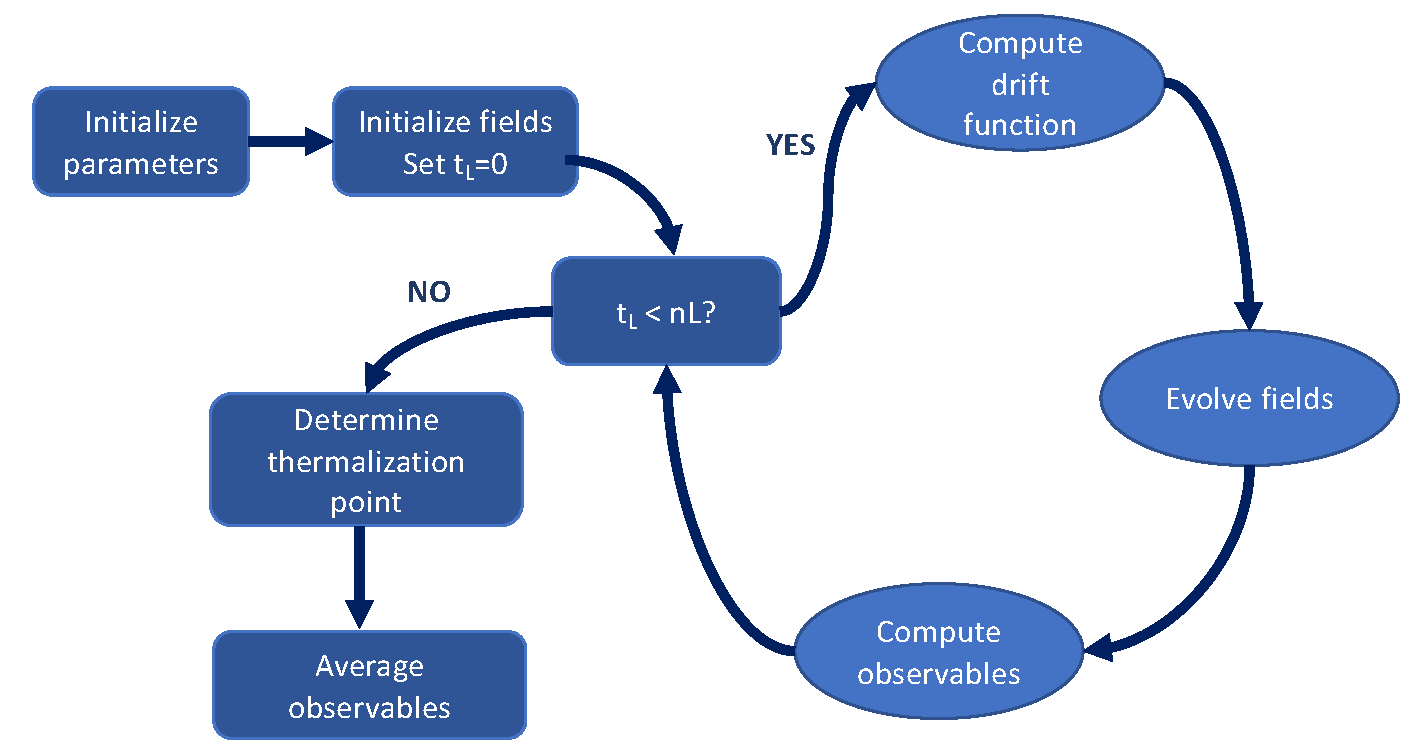
\includegraphics[width=0.6\textwidth]{./algorithm.pdf}
\caption{\label{Fig:Algorithm} Flow chart of the complex Langevin algorithm for the nonlinear sigma model.\vspace{-3mm}}
\end{figure}
\vspace{-3mm}
%
The field components are defined on a euclidean spacetime lattice, and the evolution is performed for hundreds of thousands of steps in Langevin time in order to generate enough samples to calculate observables with good statistical properties. The code for this project is written in C++ and utilizes the AMReX framework. The adaptive mesh framework in AMReX will allow us to use a nonuniform mesh to calculate the field values, which enables more efficient use of computing resources. As the lattice size grows, we concentrate our resolution in the center of the lattice, where the interesting physics will be confined due to the presence of the harmonic traps, which reduce the presence of the fields rapidly to zero outside a narrow region in the center of the trap.

\subsection{Connection to DOE Office of Science}
Previous work on this topic has been supported by the Department of Energy Computational Science Graduate Fellowship. Current work is supported under the Exascale Computing Project.

\section{Scaling and Performance}
This code uses the AMReX AMR library, which was developed at LBNL, to discretize the spacetime lattice upon which the fields are defined. While each step in Langevin time must be performed sequentially, the spacetime lattice can be updated at each of these Langevin steps in a naively parallel fashion. 
\note{a few words on AMReX and parallelization} 

Scaling results on Knights Landing (KNL) CPUs on Cori for this code are shown in Fig.~\ref{Fig:KNLScaling}.  \note{More here on scaling}
%
\vspace{-3mm}
\begin{figure}[h]
\centering
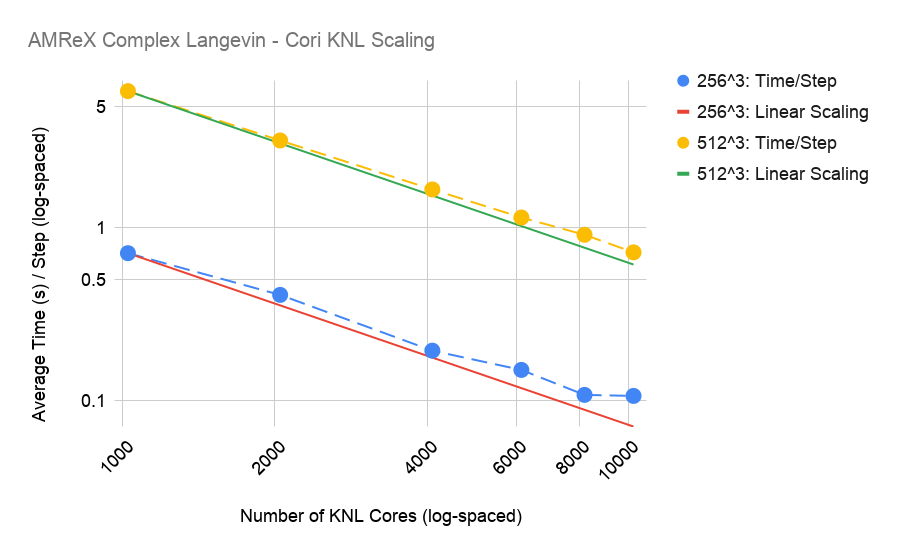
\includegraphics[width=0.6\textwidth]{./AMReX_Complex_Langevin_Cori_KNL_Scaling.png}
\caption{\label{Fig:KNLScaling} Scaling for AMReX Complex Langevin on Knights Landing CPUs.\vspace{-3mm}}
\end{figure}
\vspace{-3mm}
%
Scaling results on GPUs on Cori for this code are shown in Fig.~\ref{Fig:GPUScaling}. 
%
\vspace{-3mm}
\begin{figure}[h]
\centering
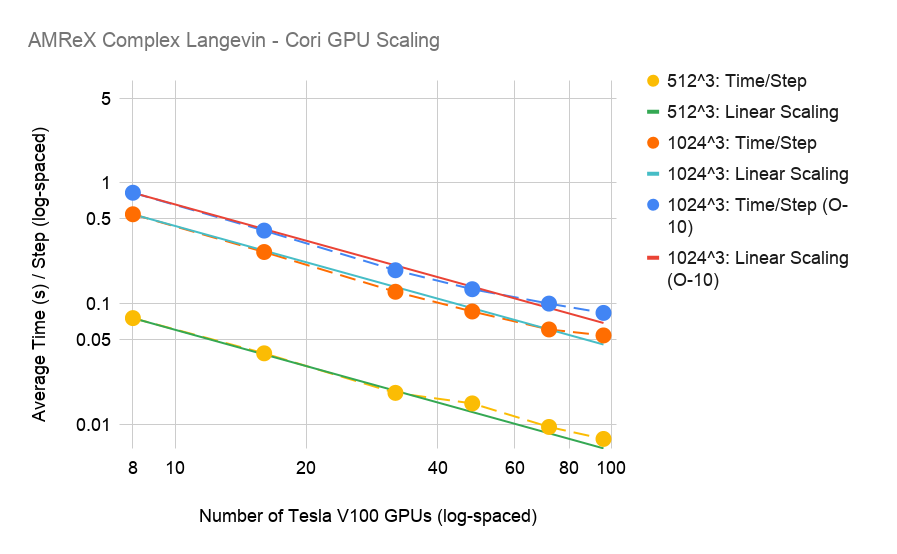
\includegraphics[width=0.6\textwidth]{./AMReX_Complex_Langevin_Cori_GPU_Scaling.png}
\caption{\label{Fig:GPUScaling} Scaling for AMReX Complex Langevin on Knights Landing CPUs.\vspace{-3mm}}
\end{figure}
\vspace{-3mm}
%



\end{document}